\documentclass[hyperref={unicode}]{beamer}
%\usecolortheme[named=Blue]{structure} % Plum, OliveGreen
\usetheme{Copenhagen} % hannover, bergen, paloalto, default
\setbeamertemplate{footline}[frame number]
\beamertemplatenavigationsymbolsempty
\usepackage[T2A]{fontenc}
\usepackage[utf8]{inputenc}
\usepackage[english,russian]{babel}

\title{Применение методов решения задачи о выполнимости булевой формулы для построения минимальной филогенетической сети}
\author[]{Мельник~М.~В.\\
Научный руководитель Ульянцев~В.~И.}
\institute{Университет~ИТМО}
\date[]{2015}


\begin{document}
\begin{frame}
  \titlepage
\end{frame}

\begin{frame}
\frametitle{Содержание}
	\tableofcontents
\end{frame}

%Обзор предметной области
\section{Обзор предметной области}

\subsection{Основные определения}

% \begin{frame}
% \frametitle{Филогенетическое дерево}

% \begin{itemize}
% 	\item Показывает историю эволюции различных видов, имеющих общего предка.
% 	\item Листья - рассматриваемые виды (таксоны).
% 	\item Вершины - эволюционное разделение.
% \end{itemize}

% \end{frame}


\begin{frame}
\frametitle{Филогенетическое дерево}

\centering

\begin{figure}[t]
	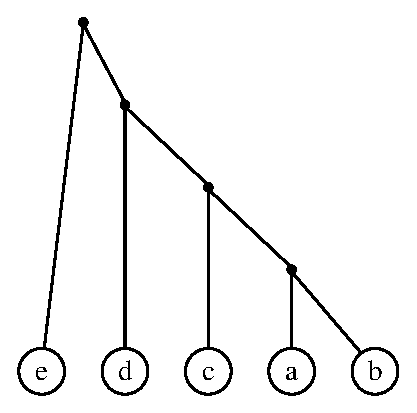
\includegraphics[width=3cm]{img/inp1.eps}
	\hspace{5mm}
	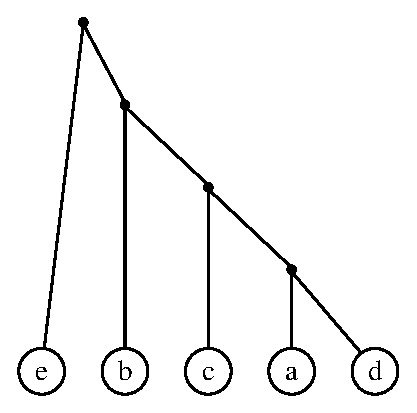
\includegraphics[width=3cm]{img/inp2.eps}
	\hspace{5mm}
	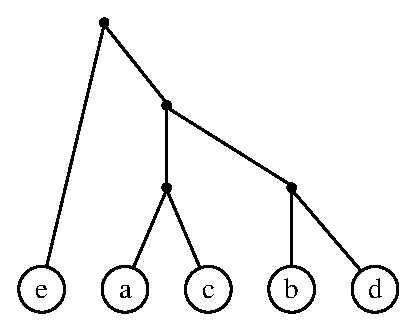
\includegraphics[width=3cm]{img/inp3.eps}
\end{figure}

Деревья над множеством таксонов \{a, b, c, d, e\}

\end{frame}

\begin{frame}
\frametitle{Филогенетическое дерево}

\textbf{Проблемы?}

Гибридную модель эволюции невозможно представить в виде филогенетических деревьев

\end{frame}

% \begin{frame}
% \frametitle{Гибридизационная сеть}

% \begin{itemize}
% 	\item Мощнее чем филогенетическое дерево.
% 	\item Ретикулярные вершины - вершины с несколькими предками. Иллюстрируют гибридизационные события.
% 	\item Может иллюстрировать любую эволюционную историю.
% \end{itemize}

% \end{frame}

\begin{frame}
\frametitle{Гибридизационная сеть}

\centering

\begin{figure}[t]
	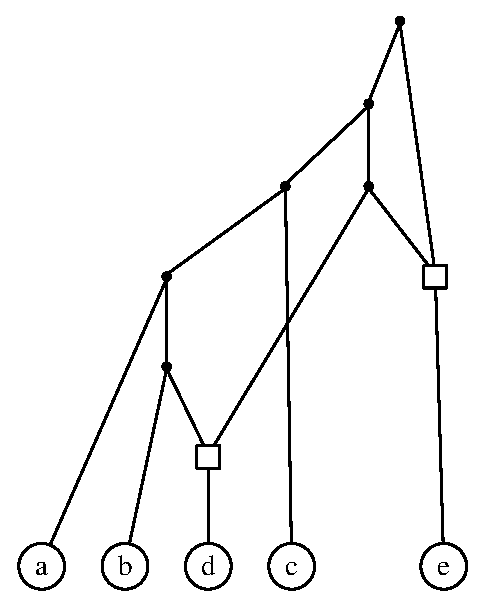
\includegraphics[width=2.8cm]{img/ans.eps}
	\hspace{1cm}
	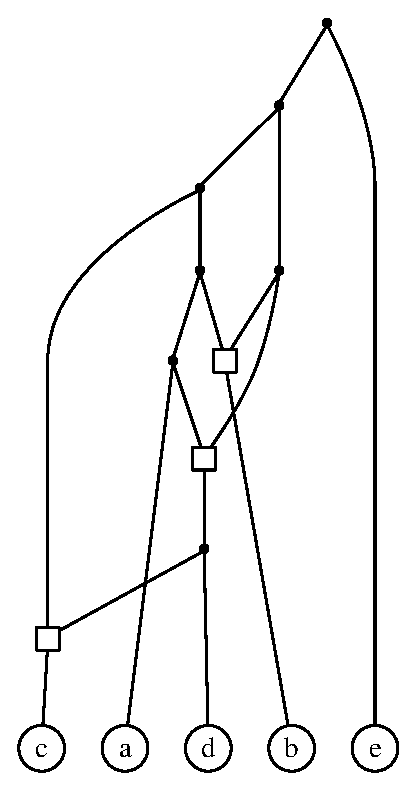
\includegraphics[width=2.8cm]{img/ans3.eps}
\end{figure}

Гибридизационные сети с двумя и тремя ретикулярными событиями соответственно

\end{frame} 

\subsection{Постановка задачи}

\begin{frame}
\frametitle{Постановка задачи}

\textbf{Построение минимальной гибридизационной сети}

По набору филогенетических деревьев построить гибридизационную сеть с наименьшим количеством вершин, которая будет отображать одновременно все деревья

\end{frame}

\begin{frame}
\frametitle{Построение минимальной гибридизационной сети}

\textbf{Мотивация}:
\begin{itemize}
	\item Маленькие гибридизационные сети проще анализировать, чем большие
	\item Принцип <<максимальной экономии>> более достоверен, чем другие (принцип наибольшего правдоподобия, принцип Байеса)
\end{itemize}


\textbf{Сложности}:
\begin{itemize}
	\item NP-полная задача
	\item Точные решения для деревьев больших размеров невозможно найти за разумное время
\end{itemize}

\end{frame}

\subsection{Существующие решения}

\begin{frame}
\frametitle{Существующие решения}

\textbf{Эвристические решения}:
\begin{itemize}
	\item $\mathrm{PIRN_{CH}}$
	\item MURPAR
	\item CASS
\end{itemize}

\textbf{Точные решения}
\begin{itemize}
	\item $\mathrm{PIRN_C}$
\end{itemize}

\end{frame}

\section{Описание алгоритма}

\begin{frame}
\frametitle{Основная идея алгоритма PhyloSAT}

Сведение к задаче о выполнимости булевой формулы

\begin{itemize}
	\item Зафиксируем количество ретикулярных событий $h$
	\item Построим булеву формулу, которая выполнима тогда и только тогда, когда существует сеть с таким количеством ретикулярных событий
	\item Проверим выполнимость формулы с помощью подходящего SAT-солвера
	\item Найдем минимальное $h$, для которого формула выполнима
\end{itemize}

\end{frame}

\begin{frame}
\frametitle{Структура сети}

Переменные для обычной вершины $v$:

\begin{itemize}
	\item $p_{v, u}$ --- $u$ является предком $v$
	\item $l_{v, u}$ --- $u$ является левым сыном $v$
	\item $r_{v, u}$ --- $u$ является правым сыном $v$
\end{itemize}

Переменные для ретикулярной вершины $v$:

\begin{itemize}
	\item $c_{v, u}$ --- $u$ является сыном $v$
	\item $p^l_{v, u}$ --- $u$ является левым предком $v$
	\item $p^r_{v, u}$ --- $u$ является правым предком $v$
\end{itemize}

Утверждения:
\begin{itemize}
	\item Уникальность детей и предков у каждой вершины
	\item Связь предков с детьми ($l_{v, u} \rightarrow p_{u, v}$ и аналогичные)
\end{itemize}

\end{frame}

\begin{frame}
\frametitle{Связь исходных деревьев с сетью}

Переменные для каждого дерева $t$:

\begin{itemize}
	\item $x_{t, v_t, v}$ --- $v$ соответствует $v_t$ в дереве $t$
	\item $a_{t, v, u}$ --- $u$ соответствует предку $v$ в дереве $t$
	\item $d_{t, v}$ --- направление предка ретикулярной вершины $v$ для отображения дерева $t$
\end{itemize}

Утверждения:
\begin{itemize}
	\item Уникальность переменных для каждой вершины и каждого дерева
	\item Трансляция связей предок--ребенок из деревьев в сеть
\end{itemize}

\end{frame}

\subsection{}

\begin{frame}
\frametitle{Дополнения и оптимизации}

\begin{itemize}
	\item Выбор SAT-солвера
	\item Быстрый поиск нижней и верхней границ $h$
	\item Поиск всех возможных решений
	\item Альтернативное сведение для уменьшения числа переменных и утверждений
\end{itemize}

\end{frame}

\section{Тестирование и результаты}

\subsection{Тестирование}

\begin{frame}
\frametitle{Методика тестирования}

\begin{itemize}
	\item Использовался набор реальных биологических данных, соответствующих злаковым травам.
	\item Для сравнения использовались алгоритмы $\mathrm{PIRN_C}$ и $\mathrm{PIRN_{CH}}$.
	\item Каждый метод запускался с ограничением времени в 1000 секунд.
\end{itemize}

\end{frame}

\begin{frame}
\frametitle{Результаты точных методов}

\begin{table}
\begin{tabular}{l | l}
	& Решено тестов \\
	\hline
	PhyloSAT & 36 \\
	PIRN$\mathrm{_C}$ & 29 \\
\end{tabular}
\end{table}

PhyloSAT быстрее на всех тестах.

\end{frame}

\begin{frame}
\frametitle{Результаты неточных методов}

\begin{table}
\begin{tabular}{l | l}
	& Решено тестов \\
	\hline
	PhyloSAT & 48 \\
	PIRN$\mathrm{_{CH}}$ & 43 \\
\end{tabular}
\end{table}

На 12 тестах, методы показали различающиеся результаты.

\begin{table}
\begin{tabular}{l | l | l}
	& Лучший результат & Лучшее время \\
	\hline
	PhyloSAT & 3 & 2 \\
	PIRN$\mathrm{_{CH}}$ & 2 & 5 \\
\end{tabular}
\end{table}

\end{frame}

%\begin{frame}
%\frametitle{Анализ нерешенных тестов}
%
%\begin{table}
%\begin{tabular}{l | l | l}
%	Тест & Полученный ответ & Нижняя граница \\
%	\hline
%	RbclRpoc & \underline{7} & \underline{7} \\
%	NdhfPhytIts & 13 & 11 \\
%	NdhfPhytRpoc & 8 & 6 \\
%	NdhfRbclRpoc & 12 & 10 \\
%	NdhfWaxyIts & 8 & 7 \\
%	PhytRbclIts & 9 & 7 \\
%	PhytRpocIts & \underline{7} & \underline{7} \\
%	RbclWaxyIts & \underline{6} & \underline{6} \\
%	NdhfPhytRbclRpoc & 9 & 7 \\
%	NdhfPhytRpocIts & 10 & 7 \\
%	NdhfRbclWaxyIts & \underline{6} & \underline{6} \\	 
%	PhytRbclRpocIts & 9 & 6 \\
%\end{tabular}
%\end{table}
%
%\end{frame}

\subsection{Примеры полученных решений}

\begin{frame}
\frametitle{Grass2WaxyIts}

\centering
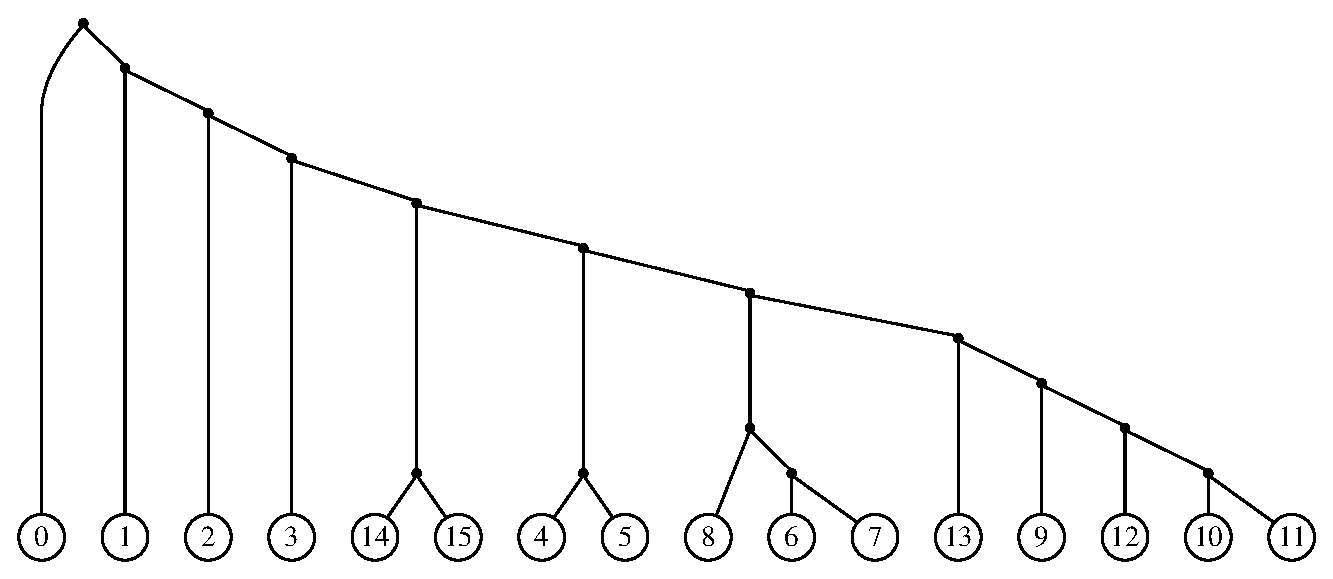
\includegraphics[width=0.87\linewidth]{img/Grass2WaxyIts_tree0}
\\
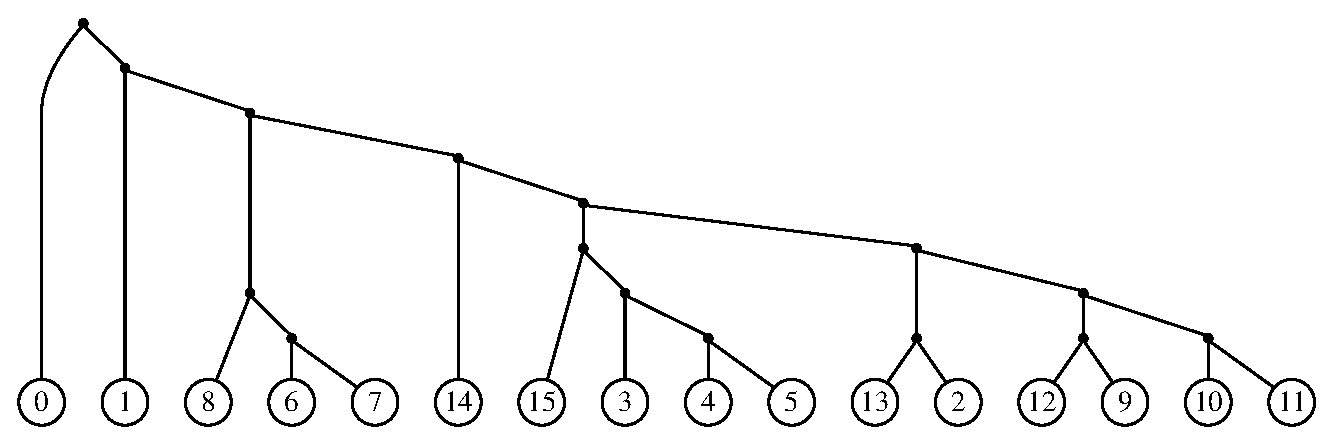
\includegraphics[width=0.87\linewidth]{img/Grass2WaxyIts_tree1}
	
\end{frame}

\begin{frame}
\frametitle{Grass2WaxyIts}

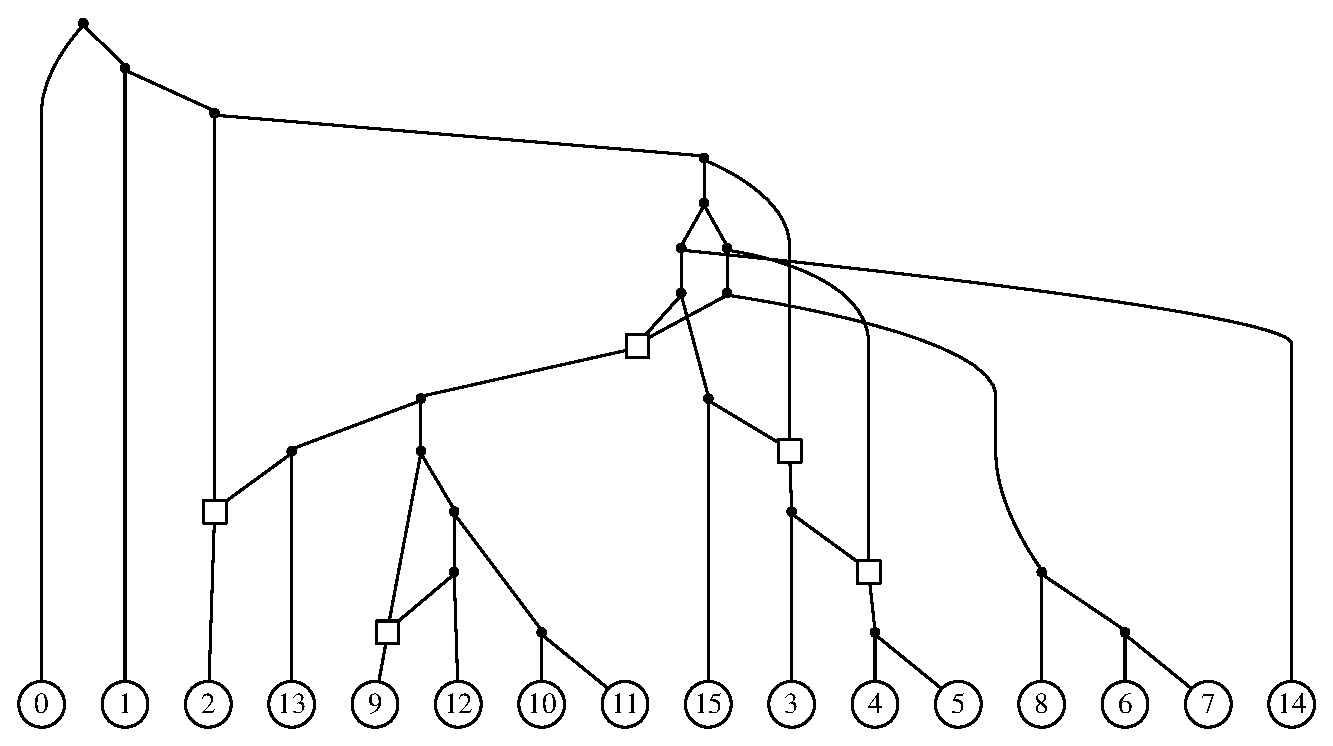
\includegraphics[width=\linewidth]{img/Grass2WaxyIts}
	
\end{frame}

\begin{frame}
\frametitle{Grass3RbclWaxyIts}

\centering
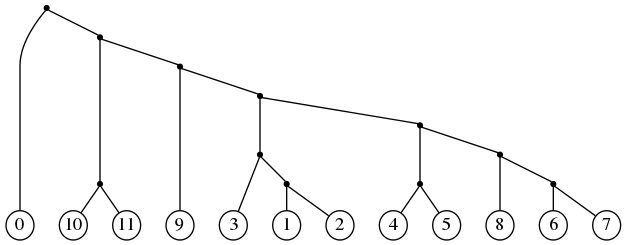
\includegraphics[width=0.54\linewidth]{img/Grass3RbclWaxyIts_tree0}
\\
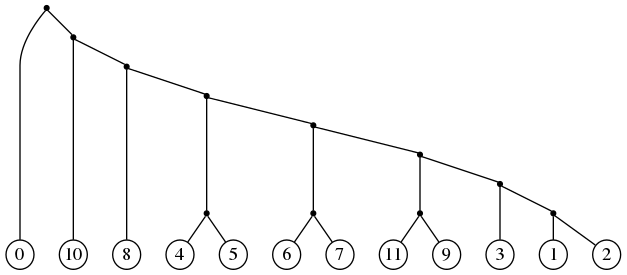
\includegraphics[width=0.54\linewidth]{img/Grass3RbclWaxyIts_tree1}
\\
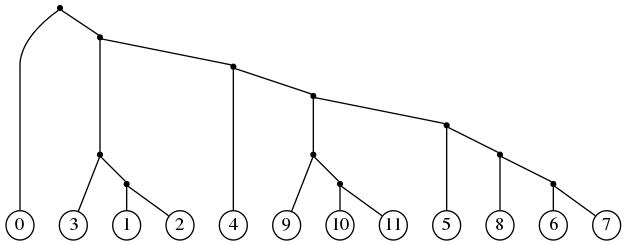
\includegraphics[width=0.54\linewidth]{img/Grass3RbclWaxyIts_tree2}

\end{frame}

\begin{frame}
\frametitle{Grass3RbclWaxyIts}

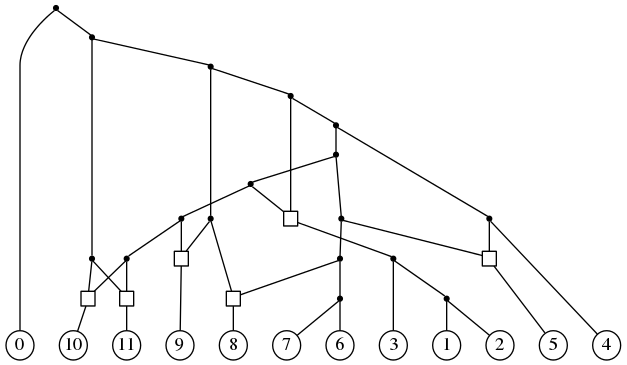
\includegraphics[width=\linewidth]{img/Grass3RbclWaxyIts}
	
\end{frame}

\section{}

\begin{frame}
\frametitle{Заключение}

Выводы:
\begin{itemize}
	\item PhyloSAT на данный момент является самым быстрым методом, гарантирующим нахождение точного решения
	\item Производительность PhyloSAT сравнима с производительностью эвристических алгоритмов
	\item Есть возможности для еще большего ускорения
\end{itemize}

Публикации:
\begin{itemize}
	\item Статья на конференцию AlCoB 2015. Мехико, Мексика, Август 4--6, 2015.
\end{itemize}

\end{frame}

\begin{frame}
\frametitle{Спасибо за внимание!}

Вопросы?

\end{frame}

\end{document}
